%نام و نام خانوادگی:
%شماره دانشجویی: 
\مسئله{else-if}

\پاسخ{}
\begin{center}
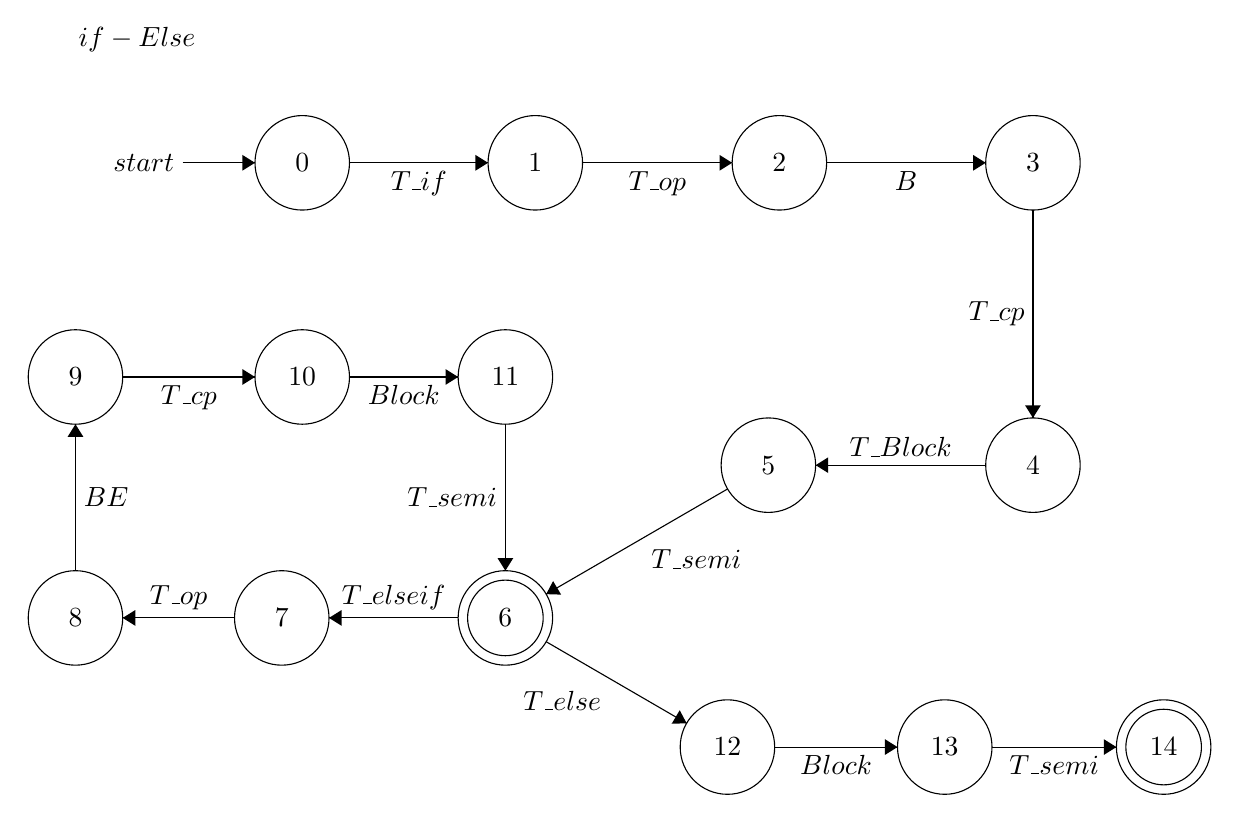
\begin{tikzpicture}[scale=0.2]
\tikzstyle{every node}+=[inner sep=0pt]

\draw (9.5,-6.9) node {$if-Else$};
\draw [black] (20,-14.7) circle (3);
\draw (20,-14.7) node {$0$};
\draw [black] (34.8,-14.7) circle (3);
\draw (34.8,-14.7) node {$1$};
\draw [black] (50.3,-14.7) circle (3);
\draw (50.3,-14.7) node {$2$};
\draw [black] (66.4,-14.7) circle (3);
\draw (66.4,-14.7) node {$3$};
\draw [black] (66.4,-33.9) circle (3);
\draw (66.4,-33.9) node {$4$};
\draw [black] (49.6,-33.9) circle (3);
\draw (49.6,-33.9) node {$5$};
\draw [black] (32.9,-43.6) circle (3);
\draw (32.9,-43.6) node {$6$};
\draw [black] (32.9,-43.6) circle (2.4);
\draw [black] (18.7,-43.6) circle (3);
\draw (18.7,-43.6) node {$7$};
\draw [black] (5.6,-43.6) circle (3);
\draw (5.6,-43.6) node {$8$};
\draw [black] (5.6,-28.3) circle (3);
\draw (5.6,-28.3) node {$9$};
\draw [black] (20,-28.3) circle (3);
\draw (20,-28.3) node {$10$};
\draw [black] (32.9,-28.3) circle (3);
\draw (32.9,-28.3) node {$11$};
\draw [black] (47,-51.8) circle (3);
\draw (47,-51.8) node {$12$};
\draw [black] (60.8,-51.8) circle (3);
\draw (60.8,-51.8) node {$13$};
\draw [black] (74.7,-51.8) circle (3);
\draw (74.7,-51.8) node {$14$};
\draw [black] (74.7,-51.8) circle (2.4);
\draw [black] (12.4,-14.7) -- (17,-14.7);
\draw (11.9,-14.7) node [left] {$start$};
\fill [black] (17,-14.7) -- (16.2,-14.2) -- (16.2,-15.2);
\draw [black] (23,-14.7) -- (31.8,-14.7);
\fill [black] (31.8,-14.7) -- (31,-14.2) -- (31,-15.2);
\draw (27.4,-15.2) node [below] {$T\_if$};
\draw [black] (37.8,-14.7) -- (47.3,-14.7);
\fill [black] (47.3,-14.7) -- (46.5,-14.2) -- (46.5,-15.2);
\draw (42.55,-15.2) node [below] {$T\_op$};
\draw [black] (53.3,-14.7) -- (63.4,-14.7);
\fill [black] (63.4,-14.7) -- (62.6,-14.2) -- (62.6,-15.2);
\draw (58.35,-15.2) node [below] {$B$};
\draw [black] (66.4,-17.7) -- (66.4,-30.9);
\fill [black] (66.4,-30.9) -- (66.9,-30.1) -- (65.9,-30.1);
\draw (65.9,-24.3) node [left] {$T\_cp$};
\draw [black] (63.4,-33.9) -- (52.6,-33.9);
\fill [black] (52.6,-33.9) -- (53.4,-34.4) -- (53.4,-33.4);
\draw (58,-33.4) node [above] {$T\_Block$};
\draw [black] (47.01,-35.41) -- (35.49,-42.09);
\fill [black] (35.49,-42.09) -- (36.44,-42.12) -- (35.93,-41.26);
\draw (45.02,-39.25) node [below] {$T\_semi$};
\draw [black] (29.9,-43.6) -- (21.7,-43.6);
\fill [black] (21.7,-43.6) -- (22.5,-44.1) -- (22.5,-43.1);
\draw (25.8,-43.1) node [above] {$T\_elseif$};
\draw [black] (15.7,-43.6) -- (8.6,-43.6);
\fill [black] (8.6,-43.6) -- (9.4,-44.1) -- (9.4,-43.1);
\draw (12.15,-43.1) node [above] {$T\_op$};
\draw [black] (5.6,-40.6) -- (5.6,-31.3);
\fill [black] (5.6,-31.3) -- (5.1,-32.1) -- (6.1,-32.1);
\draw (6.1,-35.95) node [right] {$BE$};
\draw [black] (8.6,-28.3) -- (17,-28.3);
\fill [black] (17,-28.3) -- (16.2,-27.8) -- (16.2,-28.8);
\draw (12.8,-28.8) node [below] {$T\_cp$};
\draw [black] (23,-28.3) -- (29.9,-28.3);
\fill [black] (29.9,-28.3) -- (29.1,-27.8) -- (29.1,-28.8);
\draw (26.45,-28.8) node [below] {$Block$};
\draw [black] (32.9,-31.3) -- (32.9,-40.6);
\fill [black] (32.9,-40.6) -- (33.4,-39.8) -- (32.4,-39.8);
\draw (32.4,-35.95) node [left] {$T\_semi$};
\draw [black] (35.49,-45.11) -- (44.41,-50.29);
\fill [black] (44.41,-50.29) -- (43.97,-49.46) -- (43.46,-50.32);
\draw (36.51,-48.2) node [below] {$T\_else$};
\draw [black] (50,-51.8) -- (57.8,-51.8);
\fill [black] (57.8,-51.8) -- (57,-51.3) -- (57,-52.3);
\draw (53.9,-52.3) node [below] {$Block$};
\draw [black] (63.8,-51.8) -- (71.7,-51.8);
\fill [black] (71.7,-51.8) -- (70.9,-51.3) -- (70.9,-52.3);
\draw (67.75,-52.3) node [below] {$T\_semi$};
\end{tikzpicture}
\end{center}

\pagebreak